\chapter{Inverted-Pendulum Balance Platform}\label{ch:ankle}
\graphicspath{{../Figures/40-ankle/}}

% [ZCODE 2026-10-15 Phase-A restructure: sections moved verbatim from the former monograph chapters; provenance in Notes/revision_campaign_20261015/migration_map.md]

\section{Balance Platform and Inverted-Pendulum Testbeds}\label{sec:balance_testbeds}

In parallel with the knee test stands, the author, together with McNeal and Williams, developed a family of hardware testbeds for the balance problem encountered by a humanoid: a robotic inverted pendulum actuated by BPAs at the ankle and standing on a motorized oscillating balance platform \citep{bolen_balance_2024, bolen_selfbalancing_2024, bolen_selfbalancing_srs_2024}. The testbeds deliberately reduce the robot to a single actuated joint and a single sensory question: which measurement of body orientation, fed through which feedback law, holds the leg upright on a moving support? This reduction allowed vestibular and proprioceptive feedback strategies to be exercised in hardware and provides a baseline for the full-body comparisons defined in Chapter~\ref{ch:futurework}. Three generations were built (Figure~\ref{fig:balance_inverted_pendulum}).

All three generations share one control template. A microcontroller reads body orientation, compares it against an upright set point, and commands the antagonist BPA pair with a correction proportional to the measured angle error: the command to one muscle of the pair is increased while the command to its antagonist is decreased by the same amount, about an equilibrium at which both valves sit half open, so that one muscle pressurizes as the other vents. Because the valves are on/off solenoid valves supplied from a manifold, the proportional command is realized by time-proportioning --- pulse-width modulation of the valve duty cycle --- with the switched pressure routed to the BPA chambers through a transistor-array driver stage, and with chamber pressures monitored by pneumatic pressure transducers. The pressure--force dynamics that this pulse-modulated scheme excites are modeled in companion work \citep{elzein_pressure_2025}.

The first generation used a hinge ankle driven by an antagonist pair of \qty{20}{\mm} BPAs acting as plantarflexor and dorsiflexor. Its ankle angle could be measured by a shaft encoder mounted on the hinge axis, estimated from an inertial measurement unit (IMU) mounted on the tibia, or both, selectable as the feedback source for the proportional law; the IMU angle was obtained by integrating the gyroscope angular rate after a static bias correction, with the accelerometer available as a gravity reference. The distinctive feature of this generation is its transmission. The two BPAs operated in parallel on a four-wheel block-and-tackle --- a reverse-pulley system --- mounted on the foot, with the artificial tendon reeved through the pulleys and inserting on the tibia. Reeling the tendon through the pulley train multiplies the tendon travel delivered at the joint at a proportional cost in transmitted force and an increased reaction force carried by the foot; the design consequences are examined in Section~\ref{sec:disc_error}.

The second generation, IP 2.0, replaced the hinge with a ball-and-socket ankle, so that the foot could combine plantarflexion and dorsiflexion with inversion and eversion. Three muscles were attached: one soleus-type plantarflexor, and two dorsiflexors --- one routed to act as an inverter and one as an everter --- arranged so that the muscles can act antagonistically against one another as the demanded ankle orientation changes; in the controller, the two dorsiflexors shared a single complementary command against the plantarflexor. A ball-and-socket joint presents no shaft on which a rotary encoder can be carried, so angle feedback in this generation was IMU-only.

The final balance platform stands the inverted pendulum, its ankle driven by an antagonist BPA pair, on a motorized platform that oscillates the support surface beneath the foot. An IMU on the tibia serves as a pseudo-vestibular sensor, feeding the same proportional law. This is the configuration in which balance was demonstrated both on flat ground and under the oscillating support (Section~\ref{sec:results_balance}).

\begin{figure}[htbp]
\centering
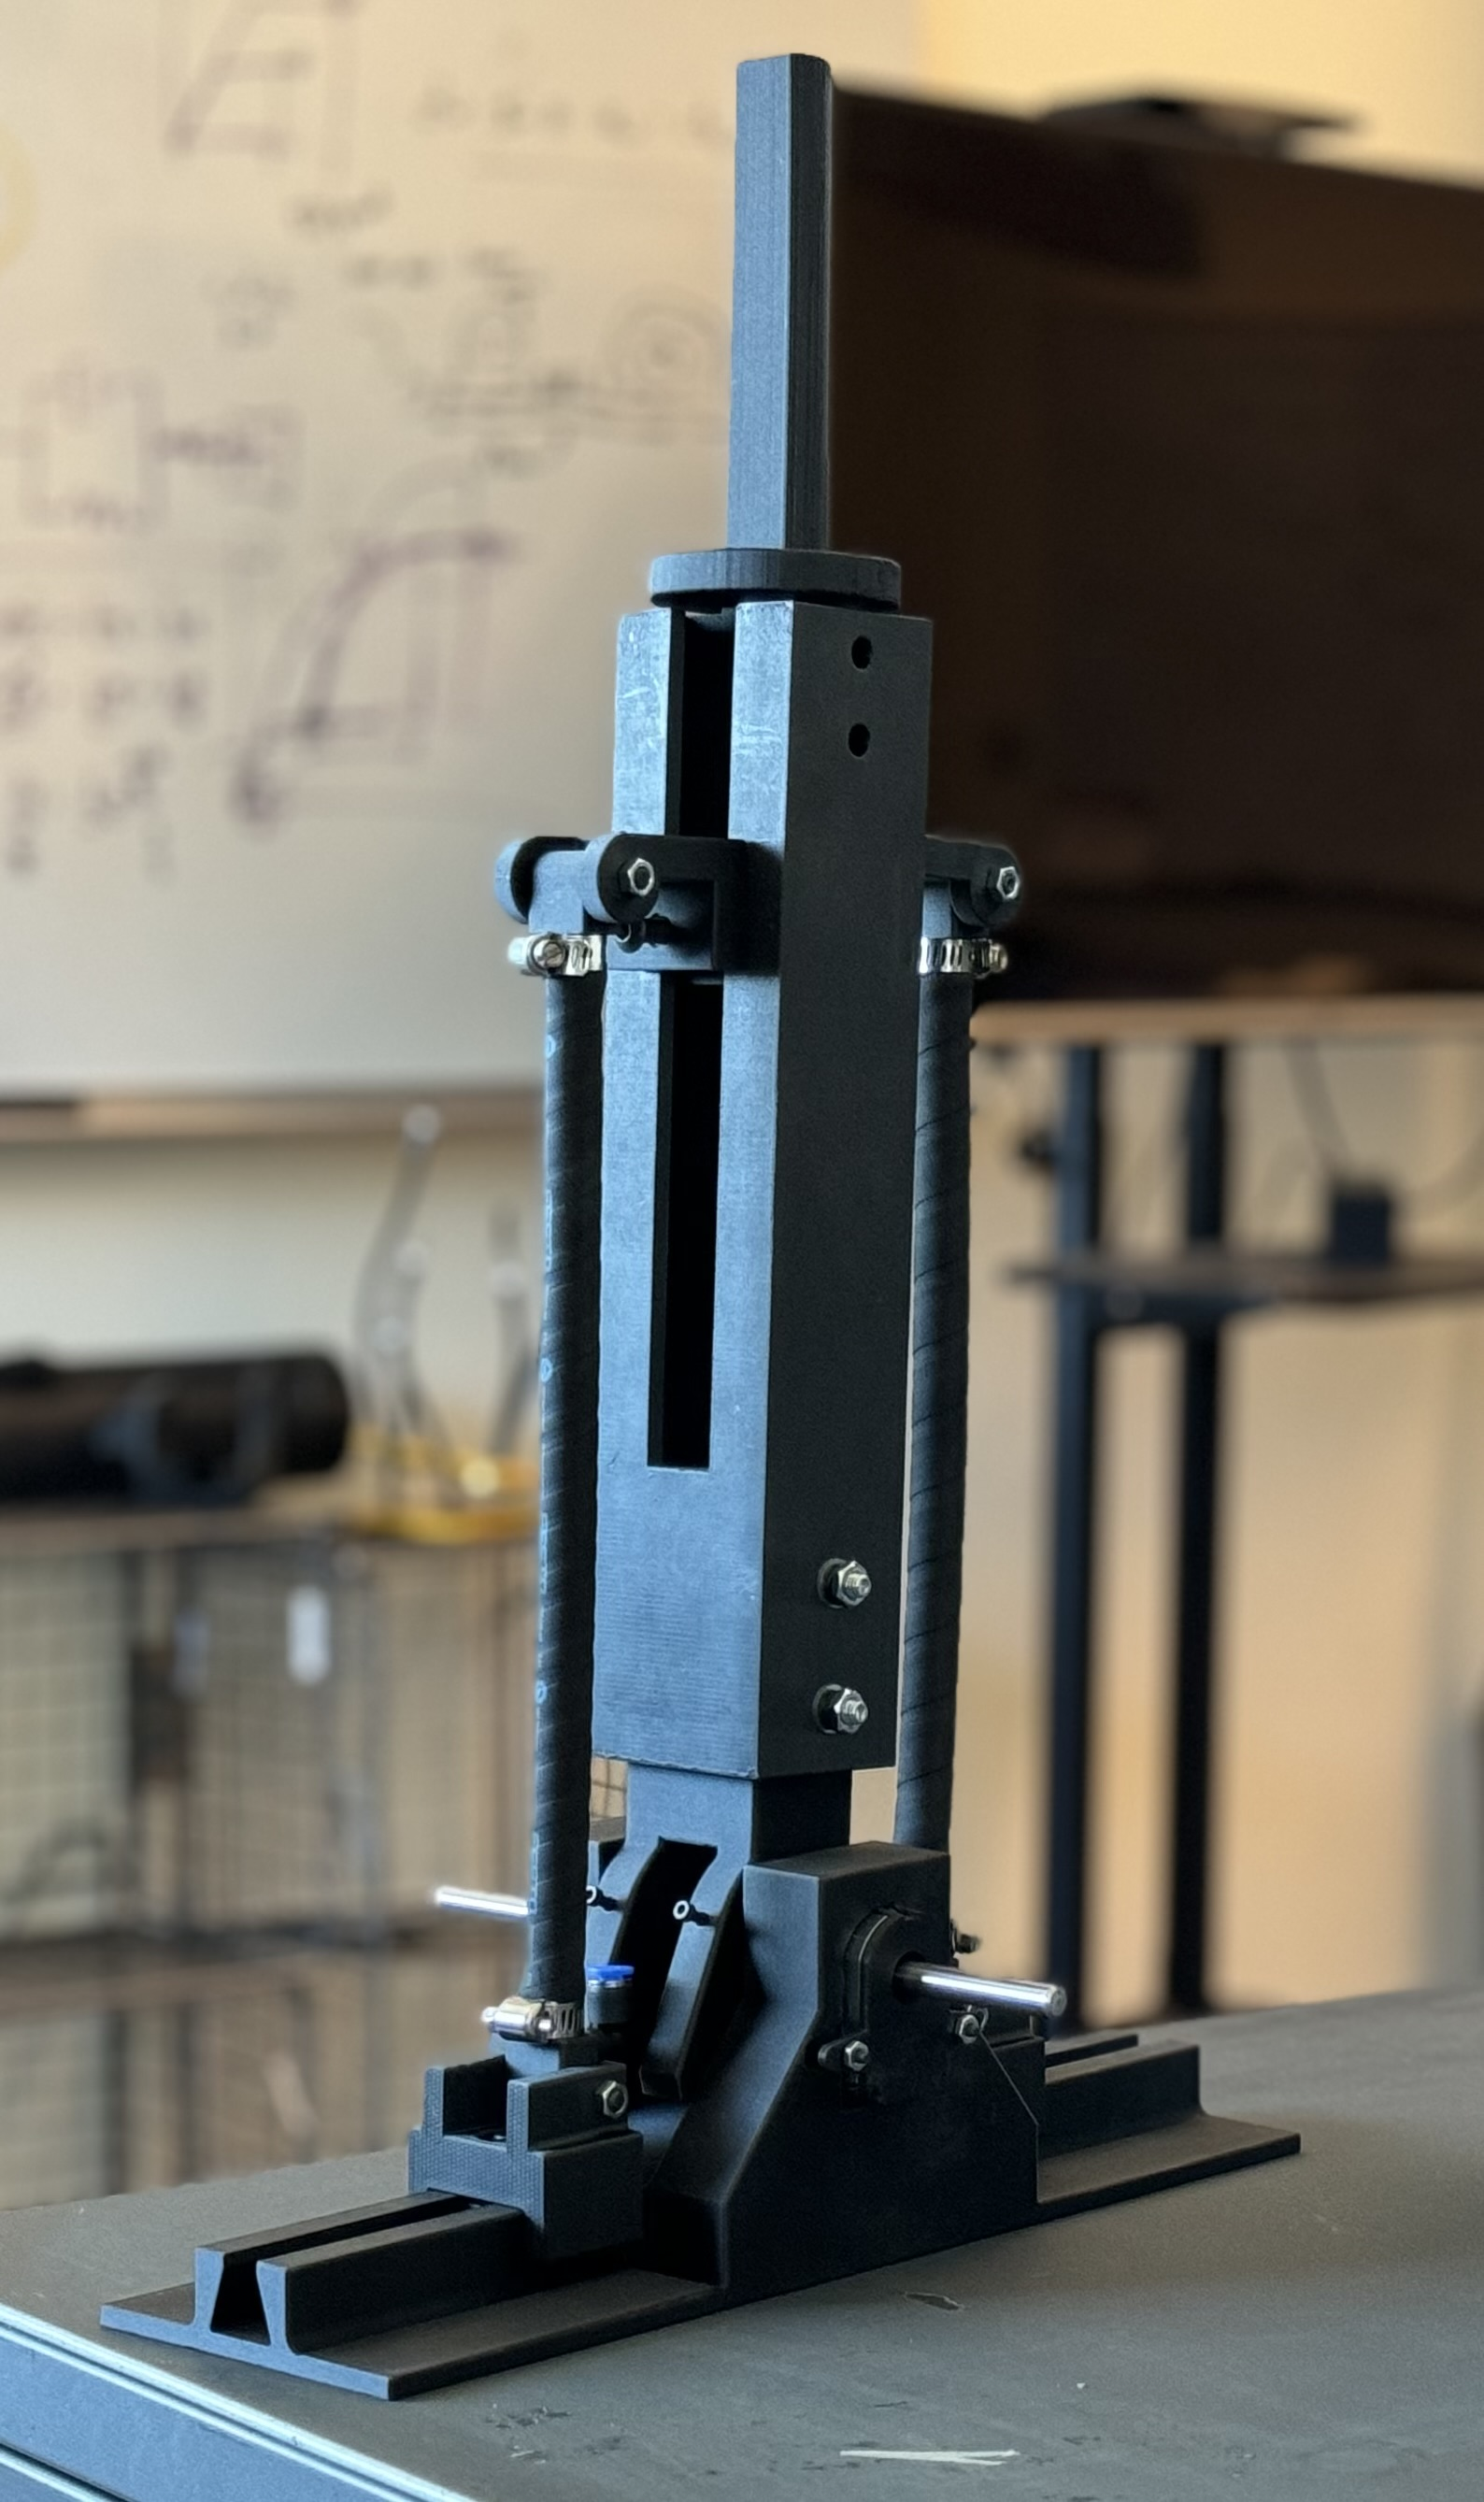
\includegraphics[width=0.60\textwidth,height=0.62\textheight,keepaspectratio]{inverted_pendulum_photo.jpg}
\caption[BPA-actuated inverted-pendulum testbed]{The BPA-actuated inverted-pendulum testbed. The pendulum shank rides on a hinge ankle above the foot assembly, and braided pneumatic actuators route down both sides of the shank to the foot, forming the antagonist ankle pair. Photograph from the AARL Inverted Pendulum project repository.}
\label{fig:balance_inverted_pendulum}
\end{figure}

\section{Balance Platform and Inverted-Pendulum Demonstrations}\label{sec:results_balance}

The testbeds of Section~\ref{sec:balance_testbeds} were demonstrated by the author and presented in three conference posters \citep{bolen_balance_2024, bolen_selfbalancing_2024, bolen_selfbalancing_srs_2024}; this section summarizes what they showed.

The first-generation pendulum --- hinge ankle, selectable encoder/IMU angle feedback, and reverse-pulley transmission --- demonstrated self-balancing: under proportional control of the antagonist \qty{20}{\mm} BPA pair with IMU pseudo-vestibular feedback, the leg held itself upright on flat ground, and balance was maintained when the same controller operated on the oscillating balance platform beneath the foot. The second generation, IP 2.0 --- ball-and-socket ankle, the three-muscle plantarflexor/inverter/everter arrangement, and IMU-only feedback --- also maintained balance, on flat terrain. Both demonstrations used the same family of Festo BPAs characterized in Section~\ref{sec:results_force}.

These demonstrations establish that balance of a BPA-actuated leg under pseudo-vestibular inertial feedback is achievable in hardware on both fixed and oscillating supports. They are reported qualitatively, however: the poster materials quote no balance durations, platform oscillation amplitudes or frequencies, ankle-angle envelopes, or valve and pressure levels, so no quantitative values are claimed here. Chapter~\ref{ch:futurework} defines an extension protocol that measures disturbance rejection, sensor drift, and sustained operation under continuous platform oscillation before comparing the same feedback architecture on a full humanoid model.

